% Full title: Spurious-Free Muller--Generalized-Bloch--Cauchy-Relation Theory Roadmap
\documentclass[UTF8,11pt,fontset=none]{ctexart}

\setCJKmainfont[BoldFont={Songti SC Bold}]{Songti SC}
\setCJKsansfont{PingFang SC}
\setCJKmonofont{PingFang SC}
\usepackage[a4paper,margin=2.05cm]{geometry}
\usepackage{amsmath,amssymb,mathtools,amsthm}
\usepackage{booktabs,longtable,tabularx,array}
\usepackage[table]{xcolor}
\usepackage{enumitem,microtype,xurl,hyperref,fancyhdr,needspace}
\usepackage{tikz}
\usetikzlibrary{arrows.meta,positioning}
\usepackage[backend=biber,style=numeric,sorting=nyt,maxbibnames=8,giveninits=true]{biblatex}
\addbibresource{references.bib}

\hypersetup{colorlinks=true,linkcolor=blue!55!black,citecolor=green!35!black,urlcolor=blue!60!black,
  pdftitle={Spurious-free Mueller--generalized-Bloch--Cauchy-relation 理论路线图},pdfauthor={TEP theory roadmap}}
\setlength{\parindent}{2em}
\setlength{\parskip}{0.25em}
\setlength{\emergencystretch}{2em}
\setlist[itemize]{leftmargin=2em,itemsep=0.2em,topsep=0.25em}
\setlist[enumerate]{leftmargin=2.2em,itemsep=0.2em,topsep=0.25em}
\renewcommand{\arraystretch}{1.16}
\newcolumntype{Y}{>{\raggedright\arraybackslash}X}
\newtheorem{theorem}{定理}
\newtheorem{proposition}[theorem]{命题}
\newtheorem{lemma}[theorem]{引理}
\theoremstyle{definition}
\newtheorem{definition}[theorem]{定义}
\newtheorem{remark}[theorem]{说明}
\newcommand{\G}{\mathcal G(k,\beta)}
\newcommand{\Cout}{\mathcal C_{\mathrm{out}}}
\newcommand{\Arel}{\mathcal A_{\mathrm{rel}}(k,\beta)}
\newcommand{\Nrep}{\mathcal N_{\mathrm{rep}}(k,\beta)}
\pagestyle{fancy}\fancyhf{}
\fancyhead[L]{Müller--generalized-Bloch--Cauchy relation 理论路线图}
\fancyhead[R]{2026-07-21}\fancyfoot[C]{\thepage}
\setlength{\headheight}{14pt}
\setcounter{tocdepth}{2}

\title{\bfseries Spurious-free Müller--generalized-Bloch--Cauchy-relation\\
周期线缺陷波导导模问题：理论研究路线图}
\author{针对 \texttt{TEP/attempt} 的可中断恢复理论规划}
\date{2026 年 7 月 21 日}

\begin{document}
\maketitle

\begin{abstract}
本报告把现有文献审计给出的主线拆成可执行的连续理论、风险门和未来离散证明链。第一阶段只研究二维标量 Helmholtz--TM 模型、光滑界面、分片常数介电系数、固定实轴向 Bloch 参数 $\beta$、严格 fixed-$\beta$ projected gap 内的实频率 $k$，并排除 Wood、threshold、unit-circle multiplier、BIC、复共振、角点、三维和非相同 leads。审计后的推荐主定理不是无条件 density uniqueness，而是
\[
 \ker\Arel/\Nrep\cong\G,
\]
其中 $\Nrep$ 是零物理重构所产生的表示零空间；仅在额外注入性成立时去掉商空间。连续链包含 15 个引理、2 个命题、3 个定理和 1 个推论；另规划 4 个离散引理和 3 个离散定理。最高风险是重构 kernel、耦合注入性及方形 Fredholm realization。报告推荐以 Package B 为承诺交付，Package A 为伸展目标，Package C 为可发表退出路线。本文只做理论规划，没有运行或实现数值实验。
\end{abstract}

\tableofcontents
\clearpage

\section{研究方向与范围}

研究对象是含有限中心缺陷区和左右周期半导的二维条带。轴向采用 $\beta$-quasiperiodic 条件，材料系数分片常数，界面和人工端口光滑。$k$ 为固定实数，严格落在完美 lead 的 fixed-$\beta$ projected spectral gap；stable/unstable multiplier clusters 与单位圆分离。第一阶段左右 leads 相同，但所有记号保留 $\pm$。

纳入：弱 TM transmission、全局 $H^1_\beta$ 导模、完整端口 Cauchy relation、Müller--Rayleigh 中心表示、generalized Bloch/Jordan trace coordinates。排除：band edge/threshold、Wood、单位圆谱、BIC/embedded mode、复频率、leaky mode、角点、三维 Maxwell 以及不同 leads。这些是第一篇论文的范围控制，不代表其不重要。

\section{当前 draft 与已有文献的关系}

当前 draft 的全局/有界问题等价应降为 restriction--gluing 引理：Fliss Theorem 4.5（SIAM JSC 35, p.~B450；本地 PDF 第 13 页）已经证明 DtN 有界化的精确等价并保持重数\cite{Fliss2013}。吸收传播/Riccati 来自 Joly--Li--Fliss Theorems 3.1、4.1（期刊 pp.~953--954）\cite{JolyLiFliss2006}，不同 leads 和误差架构见 Coatléven Theorems 4.1--4.4、5.4、5.6\cite{Coatleven2012}；DtN forbidden set 还已有 RtR 绕开方案\cite{FlissKlindworthSchmidt2015}。

当前中心表示与 Barnett--Greengard Theorem 4 和 Appendix A（期刊 pp.~6904--6906、6912--6914；Lemmas 9--10）高度重合\cite{BarnettGreengard2010}。但 draft Appendix A 的 exterior pair 混入 $D^{(nk)}$；物理 exterior double layer 必须是 $D^{(k)}$。普通 decaying Bloch vectors 的完备性陈述也应删除：Hohage--Soussi Theorem 2.2（pp.~117--118，证明 pp.~132--133）要求 generalized Floquet modes/Jordan chains，并给出 trace Riesz basis\cite{HohageSoussi2013}；Zhang 的谱分解和 modal DtN 进一步支持这一方向\cite{Zhang2021,Zhang2023}。

因此潜在创新不在任一单独组成，而在：\emph{Müller--Rayleigh quotient representation、generalized stable Cauchy traces、中心--lead 耦合及可验证的 physical-field certificate 的兼容组合}。Yuan--Lu--Antoine 已说明 BIE 单元 DtN 不是新点\cite{YuanLuAntoine2008}；Hiptmair--Moiola--Spence 则说明 second kind 不能自动排除 spurious quasi-resonance\cite{HiptmairMoiolaSpence2022}。

\section{最终目标定理}

\begin{theorem}[K1：连续 quotient-safe kernel--field equivalence]
固定满足 A1--A16 的实参数 $(k,\beta)$。设 $\Arel:\mathcal X\to\mathcal Y$ 为中心 Müller--Rayleigh 表示与左右 outgoing Cauchy relations 的耦合算子，并令
\[
\Nrep:=\ker\Arel\cap\ker\mathcal R_{\rm global}.
\]
则全局重构诱导自然线性同构
\[
 \overline{\mathcal R}_{\rm global}:\ker\Arel/\Nrep\xrightarrow{\cong}\G,
\]
并保持几何重数。在表示重构和 generalized trace synthesis 均注入的 regular subset 上，$\Nrep=\{0\}$，商空间可去掉。
\end{theorem}

正向链（completeness）为：全局场 restriction $\to$ 中心 quotient representation $\to$ 两侧 generalized stable trace coordinates $\to\ker\Arel$。反向链（soundness）为：kernel vector 重构三个区域的场 $\to$ Cauchy 匹配 $\to$ weak gluing $\to$ strict-gap decay。注入性单独由零 lead field 的 Riesz-coordinate uniqueness 与中心 $\ker\mathcal R_{\rm field}$ characterization 完成。

理想加强 T2 是 quotient realization 上 Fredholm index zero；长期加强是离散谱正确性和 no certified pollution。二者不写进 K1 的无条件前提。

\section{函数空间与基本假设}

令
\[
H^s_\beta(0,L)=\{e^{i\beta x}v:v\in H^s_{\rm per}(0,L)\},\qquad
\|u\|_{H^s_\beta}^2\asymp\sum_m\langle\beta+2\pi m/L\rangle^{2s}|u_m|^2.
\]
全局导模空间 $\G$ 定义为普通 global $H^1_\beta$ 弱核；指数横向衰减由 strict gap 推出，而非定义。pointwise decay 仅在局部椭圆正则性后陈述。端口空间为
\[
\mathcal H_\Gamma=H^{1/2}_\beta(\Gamma)\times H^{-1/2}_\beta(\Gamma),
\]
Müller densities 为 $H^{1/2}(\partial\Omega_0)\times H^{-1/2}(\partial\Omega_0)$。Rayleigh Dirichlet/Neumann coefficients 分别使用 $h^{1/2}_\beta$ 和 $h^{-1/2}_\beta$ 权重。

结构假设包括：光滑、分离的界面/端口；人工端口具有 homogeneous collar；strict projected gap；非 Wood、非 empty-cell Green pole；stable/unstable separation；half-guide trace uniqueness/closedness。representation regularity 另要求 complementary auxiliary problem 唯一，并显式排除或商掉 Calderón nullspace。Fredholm结论额外要求固定方形空间、可逆 reference operator 和 compact remainder。

\section{PDE、trace 与 gluing 证明链}

\begin{lemma}[L1--L3]
弱解具有 $H^{1/2}_\beta\times H^{-1/2}_\beta$ Cauchy traces；在 half-guide estimate 下 outgoing trace range 为闭线性子空间；restriction 与 weak gluing 在全局导模空间和中心 relation-bound solution space 之间给出同构。
\end{lemma}

关键计算是相邻子域 outward normals 相反：两侧 conormal pairing 相消才不会产生人工端口上的 distributional delta source。只匹配 Dirichlet data 不够。L3 是 Fliss Theorem 4.5 的 relation-valued 适配，不作为主要创新。若 half-guide zero-Dirichlet solution 破坏 graph uniqueness，则 relation 仍是主对象，必要时对其零迹解作商。

\section{Translation operator 与 generalized Bloch traces}

先在连续 half-guide solution/trace space 上定义一周期 translation $T^\pm$，再把 propagation operator、scattering pencil 或 ordered QZ 视为坐标 realization。在严格 projected gap 内，若 $|\lambda|=1$，则存在实 transverse quasi-momentum 的 bounded Bloch field，与 gap 矛盾；因此可用 Riesz contour 定义 stable projection。

\Needspace{10\baselineskip}
\begin{proposition}[P1：稳定广义迹表征]
在 Hohage--Soussi Theorem 2.2 的 trace-isomorphism 假设经 transmission geometry 核实后，存在包含全部 stable Jordan chains 的 Riesz synthesis $Q^\pm:\ell^2\to\mathcal H_{\Gamma^\pm}$，使
\[
 \mathcal C^\pm_{\rm out}=\operatorname{ran}Q^\pm.
\]
其 range 已闭，坐标唯一；普通 eigenvectors 的 span 不足以代替该陈述。
\end{proposition}

当 Dirichlet projection 可逆时，relation 是 $\operatorname{graph}\Lambda^\pm$；当 Robin projection 可逆时得到 RtR chart。relation 比任一 chart 基本，但不能声称 RtR 未解决 forbidden frequency。

\section{Müller--Rayleigh representation 证明链}

QP 与 free-space layer kernels 在 diagonal 具有相同 singular part；非 Wood/regular 参数下差为 smoothing。由标准 jumps 得到
\[
A_M(k,\beta)\eta+B_h(k,\beta)\xi=0,
\quad \eta=(\tau,\sigma)\in H^{1/2}\times H^{-1/2}.
\]
Barnett--Greengard 的 complementary swapped-wavenumber 架构可适配，但必须先固定 physical exterior 为 $S^{(k)},D^{(k)}$，interior 为 $S^{(nk)},D^{(nk)}$\cite{BarnettGreengard2010,ColtonKress1983}。

独立 homogeneous Rayleigh component 的作用是补足 inclusion-supported QP layers 无法生成的 empty-cell homogeneous sector。待证明的 L9 只先主张 field-surjectivity；density uniqueness 交给 L10。标准 Sobolev、弱 conormal 和 layer mapping 工具取自 McLean Chapters 3--4、6--8\cite{McLean2000}。

\section{Representation nullspace 与 spurious roots}

定义
\[
\mathcal R_{\rm field}:(\eta,\xi)\mapsto u,\qquad
\mathcal N_{\rm center}=\ker\mathcal R_{\rm field}\cap\ker[A_M\ B_h].
\]
L10 的任务是把 $\mathcal N_{\rm center}$ 写成 auxiliary complementary/Calderón projector range 的显式交或核。可能结论有三档：regular set 上为零；为有限维且可选 bounded complement；只能抽象作 quotient。物理 PDE uniqueness、field decomposition uniqueness、density uniqueness 必须分开。

Hiptmair--Moiola--Spence Theorems 1.10--1.12 和 Lemmas 2.2--2.6 表明，BIE inverse 的非物理放大可以和 physical solution operator 分离\cite{HiptmairMoiolaSpence2022}。故“second kind”及 $\sigma_{\min}\approx0$ 均不是无伪根证明。最终 certificate 必须同时检查非零重构场、PDE/interface、轴向 quasiperiodicity、两侧 port relation 和 decay。

\section{Center--lead coupled operator}

令 $x=(\eta,\xi,c^-,c^+)$，定义
\[
\Arel x=
\begin{bmatrix}
A_M\eta+B_h\xi\\
\Pi^-_\ell\eta+\Pi^-_h\xi-Q^-c^-\\
\Pi^+_\ell\eta+\Pi^+_h\xi-Q^+c^+
\end{bmatrix}.
\]
$\Pi^\pm$ 输出具有统一 outward orientation 的完整 Cauchy pair，$Q^\pm$ 合成稳定 generalized traces。每一 block 的 domain、codomain、Sobolev boundedness 和 regular component 上的 $k$-dependence 都必须单独证明。

L11 从 global field 构造 kernel class；L12 从 kernel vector 重构并 gluing；L13 证明 zero reconstructed field 只留下 $\Nrep$。其中 L13 是全路线最高风险：它同时需要 unique continuation、jump/extinction、Calderón ranges、Riesz-basis coordinate uniqueness 和 quotient geometry。

\section{Kernel--guided-space isomorphism}

K1 的 proof map 是 $[x]\mapsto u_x$；inverse 是“restriction + center representation class + two stable coordinate vectors”。L11 给出 surjectivity，L12 给出 well-defined physical range，L13 给出 injectivity modulo $\Nrep$。几何重数由线性同构保持；非线性 algebraic multiplicity 不是该结论，留待 analytic family。

与既有工作的精确边界是：Fliss 已有 PDE global/bounded equivalence，Barnett--Greengard 已有 bulk QP Müller kernel equivalence，Hohage--Soussi/Zhang 已有 generalized modal structure；K1 的候选新意仅是这些结果在 periodic line-defect center--lead relation block 中的 hypothesis-compatible quotient coupling 与 physical certificate。

\section{Fredholm framework}

L14 先证明完整 block bounded。L15 必须选择自然的方形 quotient/multitrace realization，再寻找
\[
\Arel=\mathcal A_0+\mathcal K,
\qquad \mathcal A_0^{-1}\in\mathcal L(\mathcal Y,\mathcal X),\quad
\mathcal K\ \text{compact}.
\]
候选 $\mathcal A_0$ 是 Müller/Calderón principal block 与 Riesz-normalized trace identities 的对角组合；smooth QP--free-space differences、分离曲线间 trace maps 和有限 homogeneous coupling 是 compact 候选，但必须逐项证明。

若 L15 成立，则 Kato Chapter IV 的 compact-perturbation invariance 给出 index zero\cite{Kato1995}。若 relation row 天然 rectangular、port coupling 非 compact 或 quotient 改变 index，则只保留 semi-Fredholm、closed range/finite kernel 或 finite-Rayleigh theorem。T2 是最可能失败的 theorem；失败不推翻 quotient K1。

\section{未来离散谱收敛路线}

未来定义 $\mathcal A_{N,M,h}$：$N$ 为 Nyström nodes，$M$ 为 Rayleigh cutoff，$h$ 为 cell/stable-relation discretization。证明顺序为：Müller Nyström consistency；weighted Rayleigh truncation；stable Riesz projection 的 gap convergence（含 defective clusters）；local $H^1$ reconstruction convergence；孤立 root cluster convergence；no certified pollution；edge-dependent constants。

抽象工具来自 Babuška--Osborn 和 Chatelin 的谱逼近理论\cite{BabuskaOsborn1991,Chatelin2011}，非线性 contour machinery 可参照 Beyn\cite{Beyn2012}。必须在一个不含 Green/representation/projection poles 的 contour 上取得统一 operator convergence。near-edge 常数显式依赖
\[
\delta_{\rm edge},\quad\min_j|\log|\lambda_j||,\quad
\operatorname{sep}(\sigma_s,\sigma_u),\quad\delta_{\rm Wood};
\]
这些量趋零时允许 blow-up，不承诺 threshold 上的统一定理。

\section{理论工具学习路径}

优先顺序为：A Sobolev/trace；B weak transmission/gluing；E Floquet--Bloch/Riesz traces；C layer/Calderón；D Fredholm；F invariant subspaces；G analytic operator functions；H spectral approximation。最先学习的三个模块是 A、B、E，因为它们直接控制 L1/L3 和 P1，且能在进入高风险 BIE kernel 之前确认 continuous exterior framework 是否成立。

每个模块的合格输出不是“读完”，而是能回答 gate question：弱 Neumann trace 为什么需要 PDE graph regularity；两侧 conormal 如何消掉 delta source；Jordan associated vectors 为何不能省；非零 density 如何生成零场；index 的 domain/codomain 是什么；为何 subspace gap 优于逐个 eigenvector；如何区分 operator pole 与 physical zero；何种 convergence 能排除 pollution。

\section{参考文献阅读指南}

第一阅读组：Fliss Theorems 3.5、4.5 及 Section 4；Hohage--Soussi Theorem 2.2、Lemma 5.1、Propositions 6.1--6.2；Barnett--Greengard Theorem 4 和 Appendix A。它们分别固定 PDE reduction、generalized trace basis 和 center representation 的已知边界。

第二组：Joly--Li--Fliss Theorems 3.1、4.1；Coatléven Theorems 4.1--4.4、5.4、5.6；FKS 2015 的 RtR 连续构造；Zhang 2021 Sections 3--5 和 Zhang 2023 的 modal DtN/error results。第三组：Hiptmair--Moiola--Spence Theorems 1.10--1.12、1.15 及 Section 2；McLean Chapters 3--4、6--8；Kato Chapters IV、VII；Babuška--Osborn pp.~641--787。

未核实本地全文的论文不写伪造 theorem number。所有直接引用仍必须在正式证明中逐条核对 assumptions；“相近”不等于“可套用”。

\subsection{定理依赖图}

\begin{center}
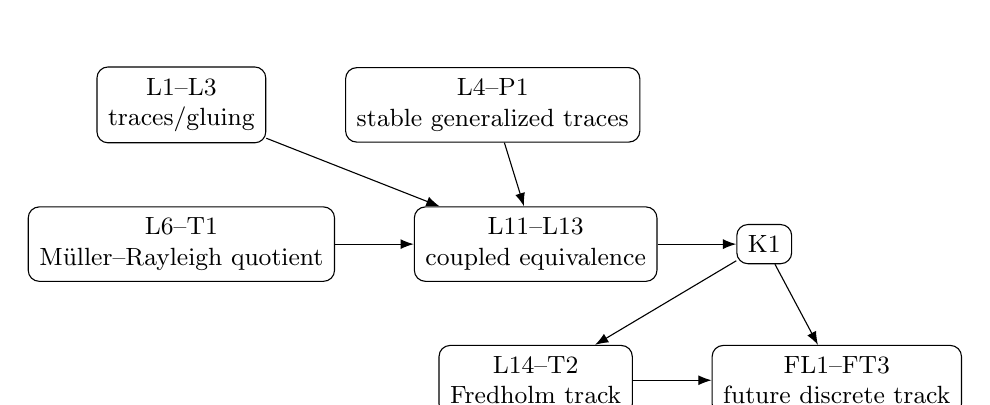
\begin{tikzpicture}[node distance=8mm and 10mm, every node/.style={draw,rounded corners,align=center,font=\small,inner sep=4pt}, >=Latex]
\node (trace) {L1--L3\\traces/gluing};
\node[right=of trace] (floquet) {L4--P1\\stable generalized traces};
\node[below=of trace] (bie) {L6--T1\\Müller--Rayleigh quotient};
\node[right=of bie] (couple) {L11--L13\\coupled equivalence};
\node[right=of couple] (main) {K1};
\node[below=of couple] (fredholm) {L14--T2\\Fredholm track};
\node[right=of fredholm] (discrete) {FL1--FT3\\future discrete track};
\draw[->] (trace)--(couple);
\draw[->] (floquet)--(couple);
\draw[->] (bie)--(couple);
\draw[->] (couple)--(main);
\draw[->] (main)--(fredholm);
\draw[->] (fredholm)--(discrete);
\draw[->] (main)--(discrete);
\end{tikzpicture}
\end{center}

前三条箭头分别提供 weak gluing、outgoing coordinate completeness 和 center quotient reconstruction；coupling 到 K1 需要 completeness/soundness/injectivity 三件事。K1 到 Fredholm 不是逻辑证明依赖，而是 physical interpretation 依赖：index zero 本身不能排除 representation roots。离散结论同时依赖连续 K1、analytic isolation 和三个 discretization components 的一致性。

\section{风险、停止条件与降级路线}

三个最高风险门为：(i) L10 找到非零 density--zero field；(ii) Hohage--Soussi trace theorem 无法适配 transmission geometry；(iii) 无自然 square $\mathcal A_0$。对应停止条件分别是：改用 quotient/side constraint；把 stable relation 作为抽象 closed subspace 或有限维 spectral projection；停止连续 T2，仅做 semi-Fredholm/finite truncation。

\begin{table}[htbp]
\centering\small
\begin{tabularx}{\textwidth}{p{0.16\textwidth}YY}
\toprule
Package & 最小可交付 & 切换条件 \\
\midrule
A 最强 & K1、index zero、continuous no-spurious、离散 convergence/no pollution & L10、L15 和 analytic approximation 均闭合 \\
B 推荐 & quotient K1、generalized stable relation、fixed-truncation injectivity、physical certificate、收敛/edge study & density uniqueness 或 continuous Fredholm 失败 \\
C 保守 & 已有 RtR/BIE，有限维 full-block reconstruction theorem，高阶 solver 与认证 & P1/K1 无法适配或被 prior art 完全覆盖 \\
\bottomrule
\end{tabularx}
\end{table}

本项目承诺 Package B，A 仅为 stretch；C 是明确可发表退出路线。完整 10 项风险登记另见伴随 \texttt{risk\_register.md}。

\section{数值实验 ToDo 占位}

本任务未运行数值实验。未来六组为：(1) random density/zero-field/complementary resonance 与 full-vs-Schur nullspace；(2) direct eig vs ordered QZ、repeated/defective multipliers、principal angles、DtN/RtR/relation conditioning；(3) Fliss geometry、圆/非圆 rods、identical leads 与 published FEM/supercell benchmark；(4) matrix/field/interface/quasiperiodic/port/decay 六重 certificate；(5) edge distance、decay exponent、spectral separation 和分项误差；(6) analytic matrix audit、mode count、pole subtraction 和 no-missed-root contour checks。

每组必须绑定理论义务：Group 1 对 L9/L10/L13，Group 2 对 L4/P1/FL3，Group 3 对 K1/FT1，Group 4 对 FT2，Group 5 对 FT3，Group 6 对 C1/FT1。任何 raw smallest singular value 都只能生成 candidate。

\section{推荐执行顺序}

第一批尝试证明 L1（Cauchy traces）、L3（restriction--gluing）和 L6（layer mappings）；它们风险低并固定记号。随后完成 Hohage--Soussi hypothesis audit，证明 L5/P1；再按 Barnett Appendix A 重做 corrected L9，但只证明 field-surjectivity。第三阶段集中攻击 L10/L13，接受 quotient。最后才尝试 L15/T2。

三个首要 proof bottlenecks 是：精确描述 $\ker\mathcal R_{\rm field}$；证明 stable generalized trace coordinates 在 transmission geometry 中注入且完备；构造方形可逆 $\mathcal A_0$ 并证明 port remainder compact。最可能失败的是 T2，而不是 quotient K1。

\section{结论}

路线图把“spurious-free”从一个矩阵口号改为可审计命题：先区分 physical field 与 density，允许 representation quotient；再用 generalized Jordan trace relation 耦合 leads；最后用双向重构和零场注入性证明 K1。当前 draft 的 restriction--gluing、QP Müller 和普通 modal completeness 均不能单独作为创新；真正可能新增的是 full coupled quotient theorem 与物理认证。

连续链计 15 lemmas、2 propositions、3 theorems、1 corollary；未来链计 4 lemmas、3 theorems。建议先学 A/B/E，先证 L1/L3/L6，主推 Package B。任何 Fredholm/no-pollution 加强都必须等待 L10、L13、L15 的严格完成。

\nocite{*}
\printbibliography[title={参考文献}]

\end{document}
